\documentclass{article}
\usepackage[ruled,vlined,linesnumbered]{algorithm2e}
\usepackage{algpseudocode}
\usepackage{amsmath}
\usepackage{amsthm}
\usepackage{graphicx}
\usepackage{subfigure}
\usepackage{float}
\usepackage{amsmath }
\usepackage{amsfonts }
\usepackage{pdfpages}
\usepackage{epsfig}
\usepackage{graphicx}
\usepackage{arydshln}
\usepackage{verbatim}
\usepackage{subfigure}
\usepackage{enumerate}
\usepackage{rotating}
\usepackage{threeparttable}
\usepackage{caption}
\usepackage{epsfig}
\usepackage{cite}
\usepackage{times}
\usepackage{geometry}
\usepackage{tikz}
\usetikzlibrary{trees}
\geometry{a4paper}
\usepackage[colorlinks,linkcolor=blue]{hyperref}
\begin{document}
\title{AI3613 Database System Concepts Homework 1}
\author{Kailing Wang 521030910356}
\date{March 22.2024}
\maketitle

\section*{Problem 1}
\begin{enumerate}[1.]
	\item
	      For the first sub-problem, we provide the result first as it is given in class as
	      \begin{align*}
		      \Pi_\text{salary}(\text{instructor}) - \Pi_\text{instructor.salary}(\text{instructor}\bowtie_\text{instructor.salary$<$d.salary} \rho_\text{d}(\text{instructor})),
	      \end{align*}
	      and simply change it to
	      \begin{align*}
		      \Pi_\text{ID, name}(\text{instructor}) - \Pi_\text{instructor.ID, instructor.name}(\text{instructor}\bowtie_\text{instructor.salary$<$d.salary} \rho_\text{d}(\text{instructor})).
	      \end{align*}

	      Expression Tree:
	      \begin{center}
		      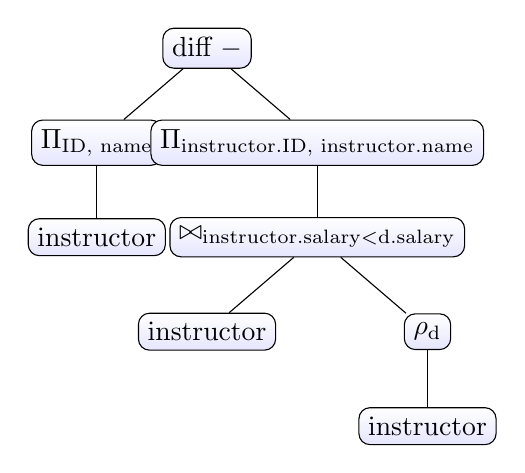
\begin{tikzpicture}[
				      every node/.style = {shape=rectangle, rounded corners,
						      draw, align=center,
						      top color=white, bottom color=blue!10},
				      level 1/.style={sibling distance=35mm},
				      level 2/.style={sibling distance=35mm},
				      edge from parent/.style={draw},
				      scale=0.8
			      ]

			      \node {diff $-$}
			      child {node {$\Pi_\text{ID, name}$}
					      child {node {instructor}}
				      }
			      child {node {$\Pi_\text{instructor.ID, instructor.name}$}
					      child {node {$\bowtie_\text{instructor.salary$<$d.salary}$}
							      child {node {instructor}}
							      child {node {$\rho_\text{d}$}
									      child {node {instructor}}
								      }
						      }
				      };
		      \end{tikzpicture}
	      \end{center}

	\item
	      Expression Tree:

	      \begin{center}
		      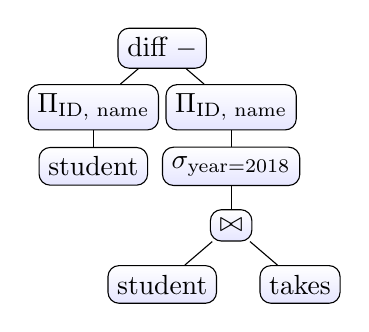
\begin{tikzpicture}[
				      every node/.style = {shape=rectangle, rounded corners,
						      draw, align=center,
						      top color=white, bottom color=blue!10},
				      level 1/.style={sibling distance=35mm},
				      level 2/.style={sibling distance=35mm},
				      edge from parent/.style={draw},
				      scale=0.5
			      ]

			      \node {diff $-$}
			      child {node {$\Pi_\text{ID, name}$}
					      child {node {student}}
				      }
			      child {node {$\Pi_\text{ID, name}$}
					      child {node {$\sigma_\text{year$=$2018}$}
							      child {node {$\bowtie$}
									      child {node {student}}
									      child {node {takes}}
								      }
						      }
				      };
		      \end{tikzpicture}
	      \end{center}

	      The expression is
	      \begin{align*}
		      \Pi_\text{ID, name}(\text{student}) - \Pi_\text{ID, name}(\sigma_\text{year$=$2018}(\text{student}\bowtie\text{takes}))
	      \end{align*}

	\item
	      Concat two advisor tables first, then select same rows with same instructor and different students.

	      Expression Tree:

	      \begin{center}
		      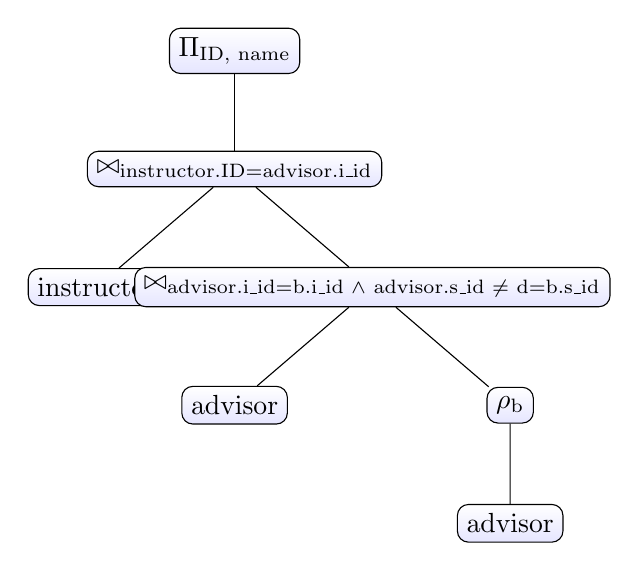
\begin{tikzpicture}[
				      every node/.style = {shape=rectangle, rounded corners,
						      draw, align=center,
						      top color=white, bottom color=blue!10},
				      level 1/.style={sibling distance=35mm},
				      level 2/.style={sibling distance=35mm},
				      edge from parent/.style={draw},
				      scale=1
			      ]

			      \node {$\Pi_\text{ID, name}$}
			      child {node {$\bowtie_\text{instructor.ID=advisor.i\_id}$}
					      child {node {instructor}}
					      child {node {$\bowtie_\text{advisor.i\_id=b.i\_id $\wedge$ advisor.s\_id $\neq$ d=b.s\_id}$}
							      child {node {advisor}}
							      child {node {$\rho_\text{b}$}
									      child	{node {advisor}}
								      }
						      }
				      };
		      \end{tikzpicture}
	      \end{center}

	      The expression is
	      \begin{align*}
		      \Pi_\text{ID, name}(\text{instructor}\bowtie_\text{instructor.ID=advisor.i\_id}(\text{advisor}\bowtie_\text{advisor.i\_id=b.i\_id $\wedge$ advisor.s\_id $\neq$ d=b.s\_id} \rho_\text{b}(\text{advisor})))
	      \end{align*}
\end{enumerate}

\section*{Problem 2}
We suppose that the operations is with DISTICT, as mentioned in calss.

From all the possible $t$s, we exlude the $t$s that do not satisfy the condition.
We cam generate all possible $t$s by $\Pi_{A_1, A_2\cdots, A_n}(R)\times S$.
The desired $t$s are in $R$, and thus the rest is
$\Pi_{A_1, A_2\cdots, A_n}(R)\times S - R$.

We simply get the desired results by a difference operation.
\begin{align*}
	\Pi_{A_1, A_2\cdots, A_n}(R) - \Pi_{A_1, A_2\cdots, A_n}(\Pi_{A_1, A_2\cdots, A_n}(R)\times S - R)
\end{align*}

\section*{Problem 3}
Let's congratulate the TAs for the second prize in the graph pattern matching competition lol.
\end{document}